\documentclass[compress]{beamer}
\usecolortheme{default}

\usepackage{lmodern, epstopdf, multirow, array, setspace, bbm, tcolorbox, pbox, bm, mathtools, tikz}
\usepackage[T1]{fontenc}

\setbeamertemplate{frametitle}[default][center]
\setbeamertemplate{footline}{\hfill \insertframenumber/\inserttotalframenumber\hspace*{5pt}\vspace{5pt}}
\setbeamertemplate{navigation symbols}{}

\newlength{\wideitemsep}
\setlength{\wideitemsep}{\itemsep}
\addtolength{\wideitemsep}{4pt}
\let\olditem\item
\renewcommand{\item}{\setlength{\itemsep}{\wideitemsep}\olditem}
\setlength{\leftmargini}{12pt}
\setlength{\leftmarginii}{14pt}
\setbeamertemplate{itemize/enumerate subbody begin}{\vspace{6pt}}
\setbeamertemplate{itemize item}[circle]
\setbeamertemplate{enumerate item}[circle]
\setbeamertemplate{enumerate subitem}[default]

\setbeamercolor{alerted text}{fg=blue}
\setbeamersize{text margin left=1.5em,text margin right=1.5em}

\tcbset{
    colback=white,
    colframe=black,
    coltext=black,
    coltitle=blue,
    colbacktitle=white,
    boxrule=1pt,
    titlerule=0pt,
    toptitle=4pt,
    top=2pt
}

\newenvironment{changemargin}[2]{% 
  \begin{list}{}{% 
    \setlength{\topsep}{0pt}% 
    \setlength{\leftmargin}{#1}% 
    \setlength{\rightmargin}{#2}% 
    \setlength{\listparindent}{\parindent}% 
    \setlength{\itemindent}{\parindent}% 
    \setlength{\parsep}{\parskip}% 
  }% 
  \item[]}{\end{list}}
  
\newenvironment{defn}{%
  \begin{tcolorbox}[title={Definition}]%
  }{\end{tcolorbox}}
  
\newenvironment{prop}[1]{%
  \begin{tcolorbox}[title={Proposition #1}]%
  }{\end{tcolorbox}}
  
\newcommand{\cit}[1]{{\footnotesize \textcolor[rgb]{0.5,0,0}{#1}}}

% Font size for code listings (verbatim blocks); reset with \normalsize
\newcommand{\codesize}{\fontsize{7}{8.5}\selectfont}

\newcommand{\slidesetup}[1]{%
  \title{#1}%
  \subtitle{\texorpdfstring{\vspace{0.3\baselineskip}}{} {\small This version: \today}}%
  \author[Mikkel Plagborg-Moller]{ECMA 31150, Spring 2026 \texorpdfstring{\\[0.5ex]}{} University of Chicago \texorpdfstring{\\[0.5ex]}{} Department of Economics \texorpdfstring{\\[4ex]}{} Mikkel Plagborg-Moller}%
  \date{}%
}

% \circleoverlay[options]{text}
% Draws a red circle with a text box nearby on a tikz overlay.
% Options (with defaults):
%   cx=0cm, cy=0cm      - circle center (shift from page center)
%   r=1cm               - circle radius
%   tx=0cm, ty=0cm      - text box offset from circle center
%   text anchor=east    - anchor of text node (east = text left, west = text right)
%   font=\normalsize    - font size for text
\pgfkeys{
  /circleoverlay/.cd,
  cx/.store in=\cocx, cx=0cm,
  cy/.store in=\cocy, cy=0cm,
  r/.store in=\cor, r=1cm,
  tx/.store in=\cotx, tx=0cm,
  ty/.store in=\coty, ty=0cm,
  text anchor/.store in=\cotextanchor, text anchor=east,
  font/.store in=\cofont, font=\normalsize,
}
\newcommand{\circleoverlay}[2][]{%
  \pgfkeys{/circleoverlay/.cd, cx=0cm, cy=0cm, r=1cm, tx=0cm, ty=0cm, text anchor=east, font=\normalsize, #1}%
  \pgfmathsetlengthmacro{\circlediameter}{2*\cor}%
  \node[draw=red, line width=2pt, circle, minimum size=\circlediameter, inner sep=0pt]
    (tmpcirc) at ([xshift=\cocx,yshift=\cocy]current page.center) {};%
  \node[anchor=\cotextanchor, fill=white, draw=red, text=red, inner sep=4pt, align=left, font=\cofont]
    at ([xshift=\cotx,yshift=\coty]tmpcirc.center) {#2};%
}

\DeclareMathOperator*{\argmax}{argmax}
\DeclareMathOperator*{\argmin}{argmin}
\DeclareMathOperator{\diag}{diag}
\DeclareMathOperator{\var}{Var}
\DeclareMathOperator{\cov}{Cov}
\DeclareMathOperator{\corr}{Corr}
\DeclareMathOperator{\lrv}{LRV}


\slidesetup{Forecasting with stationary models IV}

\begin{document}
\frame{
\maketitle
}

\frame{
\frametitle{Plan for this slide deck}
\begin{enumerate}
\item Moving average model
\item ARMA model
\item Convenient technical tool: lag polynomials
\begin{itemize}
\item Stationarity of AR($p$) model
\end{itemize}
\item AR vs.\ ARMA
\end{enumerate}
}

\frame{
\frametitle{Moving average model}
\begin{itemize}
\item In an AR model, current outcomes depend on lagged outcomes.
\item Different way to model time series dependence: lagged innovations instead of lagged outcomes.
\[y_t = \mu + u_t + \theta u_{t-1},\]
where $u_t$ is a white noise process with variance $\sigma_u^2$: $u_t \sim \mathit{WN}(\sigma_u^2)$.
\item Called a \textbf{moving average} (MA).
\item We can generalize to $q$ lagged innovations: MA($q$).
\[y_t = \mu + u_t + \theta_1 u_{t-1} + \dots + \theta_q u_{t-q}.\]
\item Always cov.\ stationary, regardless of the parameters $\theta_1,\dots,\theta_q,\sigma_u^2$.
\end{itemize}
}

\frame{
\frametitle{MA($q$) model: ACF}
\[y_t = \mu + u_t + \theta_1 u_{t-1} + \dots + \theta_q u_{t-q},\quad u_t \sim \mathit{WN}(\sigma_u^2)\]
\begin{itemize}
\item Clearly, $E(y_t) = \mu$.
\item \alert{Exercise:} show
\[\gamma(\ell) \equiv \cov(y_t,y_{t-\ell}) = \begin{cases}
\sigma_u^2\sum_{j=0}^{q-\ell} \theta_j \theta_{j+\ell} & \text{for } 0 \leq \ell \leq q, \\
0 & \text{for } \ell>q,
\end{cases}\]
where $\theta_0 \equiv 1$.
\item The process exhibits \textbf{finite dependence}: autocorrelations are exactly zero after $q$ lags (unlike AR processes).
\end{itemize}
}

\frame{
\begin{figure}
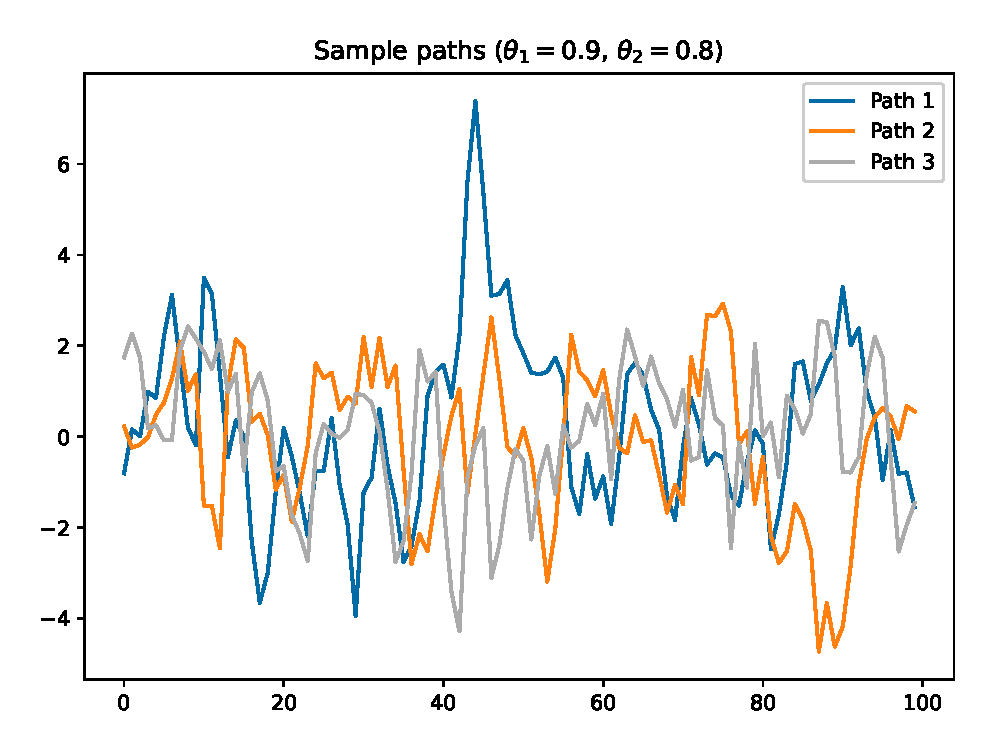
\includegraphics[width=0.9\linewidth]{fig/ma_sim.eps}
\[y_t = u_t + \theta_1 u_{t-1} + \theta_2 u_{t-2},\quad u_t \overset{iid}{\sim} N(0,1),\quad \theta_1=0.9,\,\theta_2=0.8\]
\end{figure}
}

\frame{
\begin{figure}
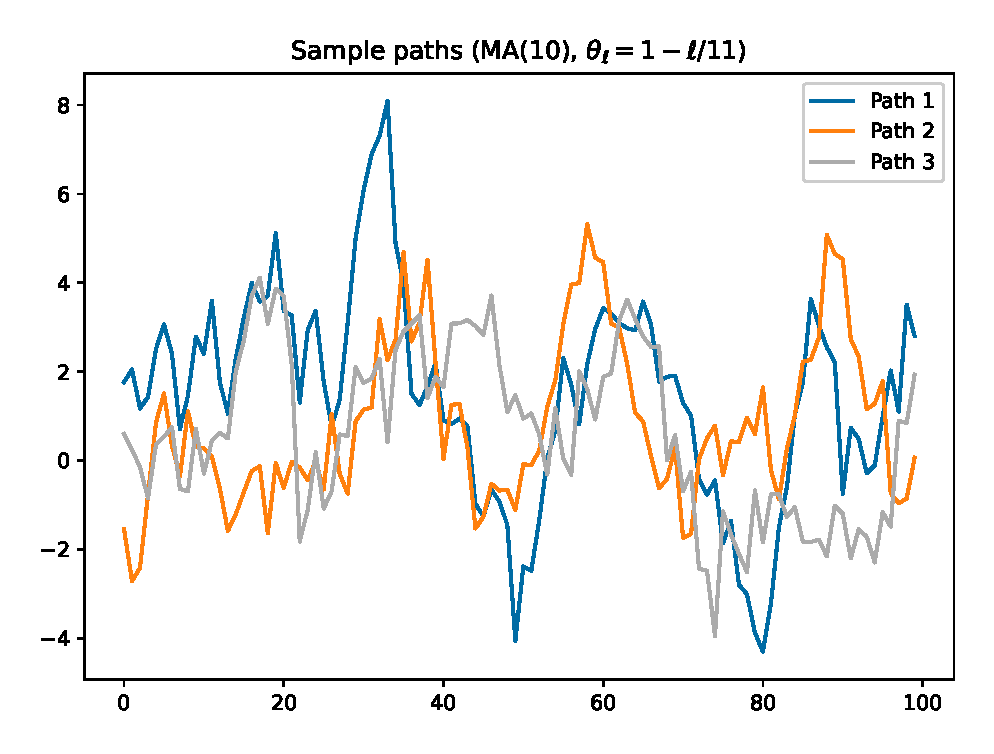
\includegraphics[width=0.9\linewidth]{fig/ma10_sim.eps}
\[y_t = u_t + \sum_{\ell=1}^{10} \theta_\ell u_{t-\ell},\quad u_t \overset{iid}{\sim} N(0,1),\quad \theta_\ell=1-\tfrac{\ell}{11}\]
\end{figure}
}

\frame{
\frametitle{Wold decomposition}
\begin{itemize}
\item MA processes turn out to be very general.
\item \alert{Result} (\textbf{Wold decomposition}): any cov.\ stationary time series $\lbrace y_t \rbrace$ can be arbitrarily well approximated as $q \to \infty$ by
\[y_t = \zeta_t + u_t + \sum_{\ell=1}^q \theta_\ell u_{t-\ell}, \quad \text{where:}\]
\vspace{-\baselineskip}
\begin{itemize}
\item $u_t$ is some white noise process.
\item $\zeta_t$ is a perfectly predictable process (typically just a constant mean).
\end{itemize}
\item If the autocovariances of $\lbrace y_t \rbrace$ satisfy $\gamma(\ell)=0$ for all $\ell>m$ (finite dependence), then $y_t$ can be represented as an MA($m$) process (plus perfectly predictable part).
\item But if the ACF decays slowly to zero, then we may need large $q$ to get a good approximation.
\end{itemize}
}

\frame{
\frametitle{ARMA($p,q$) model}
\begin{itemize}
\item We can combine the AR and MA modeling frameworks:
\[y_t = c + a_1 y_{t-1} + \dots + a_p y_{t-p} + u_t + \theta_1 u_{t-1} + \dots + \theta_q u_{t-q},\]
\[u_t \sim \mathit{WN}(\sigma_u^2).\]
\item Called an \textbf{ARMA($p,q$) model}.
\begin{itemize}
\item $p$ AR lags.
\item $q$ MA lags.
\end{itemize}
\item Rich modeling framework for capturing stationary time series dynamics.
\end{itemize}
}

\frame{
\begin{figure}
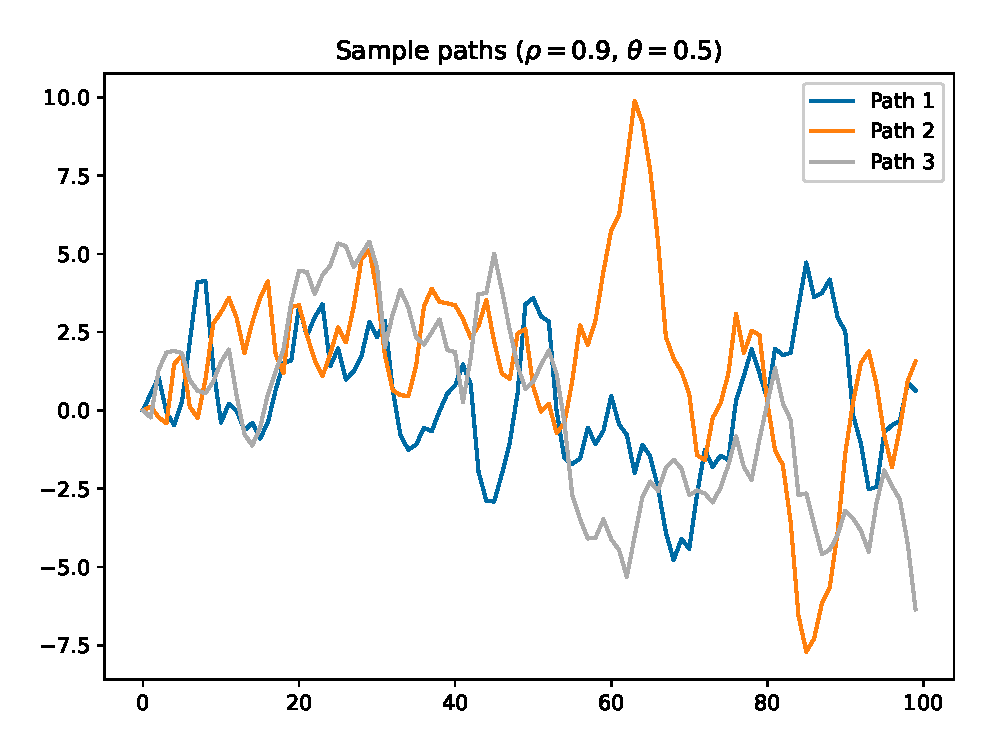
\includegraphics[width=0.9\linewidth]{fig/arma_sim.eps}
\[y_t = \rho y_{t-1} + u_t + \theta u_{t-1},\quad u_t \overset{iid}{\sim} N(0,1),\quad \rho=0.9,\,\theta=0.5\]
\end{figure}
}

\frame{
\frametitle{Loose ends}
\begin{itemize}
\item We have some loose ends:
\begin{enumerate}
\item When is an AR/ARMA process covariance stationary?
\item How do we forecast an ARMA($p,q$) process?
\item How to estimate ARMA parameters?
\end{enumerate}
\item To make progress on {\#}1--2, it's helpful to work with lag polynomials (next slides).
\item We will tackle {\#}3 much later when we talk about state space models.
\end{itemize}
}

\frame{
\frametitle{Lag operator}
\begin{itemize}
\item It's convenient to use the \textbf{lag operator} notation
\[Ly_t \equiv y_{t-1}.\]
The operator $L$ replaces a time series $\lbrace y_t \rbrace$ with its lag $\lbrace y_{t-1} \rbrace$.
\item Applying it twice, we get the second lag:
\[L^2y_t = L(Ly_t) = Ly_{t-1} = y_{t-2}.\]
\item And so on:
\[L^\ell y_t = y_{t-\ell}.\]
\item Negative powers give leads:
\[L^{-\ell}y_t = y_{t+\ell}.\]
\item And $L^0$ is the identity operator:
\[L^0y_t = y_t.\]
\end{itemize}
}

\frame{
\frametitle{Lag polynomial}
\begin{itemize}
\item We can now define a $p$-th order \textbf{lag polynomial}:
\[b(L) = b_0 + b_1 L + \dots + b_p L^p = \sum_{\ell=0}^p b_\ell L^\ell.\]
\item This just means that
\[b(L)y_t = b_0 y_t + b_1 y_{t-1} + \dots + b_p y_{t-p} = \sum_{\ell=0}^p b_\ell y_{t-\ell}.\]
\item We also call a lag polynomial a \textbf{linear filter}.
\item If $\lbrace y_t \rbrace$ is covariance stationary, then so is $b(L)y_t$.
\end{itemize}
}

\frame{
\frametitle{Two-sided linear filters}
\begin{itemize}
\item We can generalize to a \textbf{two-sided} linear filter:
\[b(L) = \sum_{\ell=-p}^p b_\ell L^\ell \quad \Longrightarrow \quad b(L)y_t = \sum_{\ell=-p}^p b_\ell y_{t-\ell} \quad \text{(lags and leads)}.\]
(If $b_\ell=0$ for $\ell<0$, the filter is \textbf{one-sided}.)
\item Examples of linear filters:
\begin{itemize}
\item First difference: $b(L)y_t = \Delta y_t \equiv y_t - y_{t-1}$ ($b_0=1,b_1=-1$).
\item One-year change (monthly data): $b(L)y_t = y_t - y_{t-12}$ ($b_0=1,b_1=\dots=b_{11}=0,b_{12}=-1$).
\item Three-period central moving average: $b(L)y_t = (y_{t-1}+y_t+y_{t+1})/3$ ($b_{-1}=b_0=b_1=1/3$).
\end{itemize}
\end{itemize}
}

\frame{
\frametitle{Multiplication of lag polynomials}
\begin{itemize}
\item Start with a time series that's a linear filter:
\[y_t = b(L)u_t,\quad \text{with}\quad b(L)=\sum_{\ell=-p}^p b_\ell L^\ell.\]
\item Now take a linear filter $d(L)=\sum_{\ell=-q}^q d_\ell L^\ell$ of that series:
\[z_t = d(L)y_t = g(L)u_t,\quad \text{where} \quad g(L) \equiv d(L)b(L).\]
\item $g(L) = \sum_{\ell=-(p+q)}^{p+q} g_\ell L^\ell$ is a linear filter of order $p+q$.
\begin{itemize}
\item \alert{Exercise:} what are its coefficients $g_\ell$?
\end{itemize}
\item Facts:
\begin{enumerate}
\item $b(L)d(L)=d(L)b(L)$.
\item If $d$ is a constant, $b(L)d = b(1)d = d\sum_{\ell=-p}^p b_\ell$.
\end{enumerate}
\end{itemize}
}

\frame{
\frametitle{Example: multiplication of lag polynomials}
\[y_t \equiv \Delta u_t = (1-L)u_t\]
\[z_t \equiv \Delta y_t = (1-L)y_t = (1-L)^2u_t\]
\[(1-L)^2 = 1-2L+L^2\]
\[\Downarrow\]
\[z_t = u_t -2u_{t-1} + u_{t-2}\]
}

\frame{
\frametitle{AR($p$): towards stationarity}
\begin{itemize}
\item Now let's use lag polynomials to analyze the AR($p$) model:
\[y_t = c + a_1 y_{t-1} + a_2 y_{t-2} + \dots + a_p y_{t-p} + u_t.\]
\item Using our new notation, we can write this compactly:
\[a(L)y_t = c + u_t,\quad \text{where} \quad a(L) \equiv 1-\sum_{\ell=1}^p a_\ell L^\ell.\]
\item \emph{Suppose} we could find a one-sided lag polynomial $b(L)$ such that $b(L)a(L)=1$. Then
\[y_t = b(L)a(L)y_t = b(L)(c + u_t).\]
$\Longrightarrow$ $y_t$ is a one-sided linear filter of the white noise process $u_t$ \newline
$\Longrightarrow$ $y_t$ is cov.\ stationary.
\end{itemize}
}

\frame{
\frametitle{Inverse of lag polynomial}
\begin{itemize}
\item A one-sided lag polynomial $b(L)$ satisfying $b(L)a(L)=1$ is called the \textbf{inverse} of $a(L)$, written $b(L)=a(L)^{-1}$.
\item \alert{Result:} $a(L)=1-\sum_{\ell=1}^p a_\ell L^\ell$ has a one-sided inverse, $a(L)^{-1}$, if all the complex solutions of the \textbf{characteristic equation}
\[a(z)=0\]
lie outside the unit circle, i.e., $|z|>1$.
\item Writing out the characteristic equation explicitly:
\[a_1 z + a_2 z^2 + \dots + a_p z^p = 1.\]
This has exactly $p$ complex solutions (fundamental theorem of algebra). If they're all larger than 1 in modulus, then $a(L)^{-1}$ exists.
\end{itemize}
}

\frame{
\frametitle{Technical detail: infinite-order lag polynomials}
\begin{itemize}
\item The inverse $b(L) = \sum_{\ell=0}^\infty b_\ell L^\ell = a(L)^{-1}$ might be of \textbf{infinite order}, i.e., $b_\ell \neq 0$ even for large $\ell$.
\item Not a mathematical problem: everything we've said goes through when the lag polynomial has $\infty$-ly many terms.
\item There is one requirement though: for an infinite-order polynomial $b(L) = \sum_{\ell=0}^\infty b_\ell L^\ell$ to yield a mathematically well-defined process $b(L)y_t$ for any cov.\ stationary $\lbrace y_t \rbrace$, its coefficients must be \textbf{absolutely summable}:
\[\sum_{\ell=0}^\infty |b_\ell|<\infty.\]
\item Thankfully, if the characteristic equation $a(z)=0$ has all solutions outside the unit circle, then there does indeed exist a one-sided $a(L)^{-1}$ with absolutely summable coefficients.
\end{itemize}
}

\frame{
\frametitle{AR($p$): stationary condition}
\begin{itemize}
\item To summarize, we've seen that the AR($p$) model
\[y_t = c + a_1 y_{t-1} + a_2 y_{t-2} + \dots + a_p y_{t-p} + u_t,\quad u_t \sim \mathit{WN}(\sigma_u^2),\]
has a cov.\ stationary solution $\lbrace y_t \rbrace$ when the characteristic equation
\[a(z)=1-\sum_{\ell=1}^p a_\ell z^\ell=0\]
has all its solutions $z$ (called \textbf{roots}) outside the unit circle.
\item Moreover, in this case,
\[y_t = a(L)^{-1}(c+u_t) = \frac{c}{1-\sum_{\ell=1}^p a_\ell} + a(L)^{-1}u_t,\]
so $\lbrace y_t \rbrace$ is also an $\infty$-order MA process.
\end{itemize}
}

\frame{
\frametitle{Special case: AR(1)}
\[y_t = c + \rho y_{t-1} + u_t\]
\vspace{-0.5\baselineskip}
\begin{itemize}
\item Characteristic equation:
\[\rho z = 1 \quad \Longrightarrow \quad z = \frac{1}{\rho}.\]
So $|z|>1$ if and only if $|\rho|<1$. Same as we derived previously!
\item Inverse of AR polynomial:
\[(1-\rho L)^{-1} = \sum_{\ell=0}^\infty (\rho L)^\ell \quad \text{(geometric series)}.\]
\item So $y_t$ has the MA representation
\[y_t = (1-\rho L)^{-1}(c+u_t) = \boxed{\frac{c}{1-\rho} + \sum_{\ell=0}^\infty \rho^\ell u_{t-\ell}}. \]
\end{itemize}
}

\frame{
\frametitle{Special case: AR(1) -- continued}
\begin{itemize}
\item We could also have obtained the MA representation by repeated substitution in the AR equation:
\begin{align*}
y_t &= c + \rho y_{t-1} + u_t \\
&= c + \rho(c + \rho y_{t-2} + u_{t-1}) + u_t \\
&= c + \rho(c + \rho (c + \rho y_{t-3} + u_{t-2}) + u_{t-1}) + u_t \\
&\vdots
\end{align*}
\item \dots but the lag polynomial method is much simpler and more generalizable when you get used to the mechanics.
\end{itemize}
}

\frame{
\frametitle{ARMA models: stationarity and invertibility}
\begin{itemize}
\item Write an ARMA($p,q$) model compactly using lag polynomials:
\[a(L)y_t = c + \theta(L)u_t,\quad a(L) \equiv 1 - \sum_{\ell=1}^p a_\ell L^\ell,\quad \theta(L) \equiv 1 + \sum_{\ell=1}^q \theta_\ell L^\ell.\]
\item If $a(L)$ is invertible, then
\[y_t = \mu + d(L)u_t,\quad \text{where}\quad d(L) \equiv a(L)^{-1}\theta(L),\quad \mu \equiv a(1)^{-1}c,\]
so $y_t$ is a (cov.\ stationary) MA($\infty$) process.
\item If $\theta(L)$ is invertible, then
\[u_t = \psi(L)(y_t-\mu),\quad \text{where} \quad \psi(L) \equiv \theta(L)^{-1}a(L),\]
and $u_t$ is \textbf{invertible}: function of current and lagged $y_t,y_{t-1},y_{t-2},\dots$, but not of future $y_{t+1},y_{t+2},\dots$.
\end{itemize}
}

\frame{
\frametitle{ARMA models: forecasting}
\[y_t = c + \sum_{\ell=1}^p a_\ell y_{t-\ell} + u_t + \sum_{\ell=1}^q \theta_\ell u_{t-\ell},\quad E[u_t \mid \lbrace y_s \rbrace_{s<t}]=0\]
\begin{itemize}
\item Assume the ARMA model is cov.\ stationary and invertible. Then
\[u_{t-\ell} = \psi(L)(y_{t-\ell}-\mu) \quad \text{(function of } y_{t-\ell},y_{t-\ell-1},\dots \text{)}.\]
\item Best one-step-ahead forecast:
\[E[y_t \mid y_{t-1},y_{t-2},\dots] = c + \sum_{\ell=1}^p a_\ell y_{t-\ell} + \sum_{\ell=1}^q \theta_\ell \psi(L)(y_{t-\ell}-\mu).\]
\item In general, this depends on $\infty$-ly many lags $y_{t-1},y_{t-2},\dots$, not just a finite number $p$ like for AR($p$) models.
\end{itemize}
}

\frame{
\frametitle{Forecasting example: MA(1)}
\[y_t = u_t + \theta u_{t-1} = \theta(L)u_t,\quad \theta(L) \equiv 1+\theta L\]
\begin{itemize}
\item If $|\theta|<1$, then
\[\theta(L)^{-1} = \sum_{\ell=0}^\infty (-\theta L)^\ell \quad \text{(geometric series)}\]
\[\Downarrow\]
\[u_t = \theta(L)^{-1} y_t = \sum_{\ell=0}^\infty (-\theta)^\ell y_{t-\ell}\]
\[\Downarrow\]
\begin{align*}
&E[y_t \mid y_{t-1},y_{t-2},\dots] = \theta \times E[u_{t-1} \mid y_{t-1},y_{t-2},\dots] \\
&=\theta \times \theta(L)^{-1} y_{t-1} = \boxed{\theta y_{t-1} - \theta^2 y_{t-2} + \theta^3 y_{t-3} - \dots}
\end{align*}
\end{itemize}
}

\frame{
\frametitle{AR or ARMA?}
\begin{itemize}
\item ARMA models can capture complicated dynamics, but difficult to estimate/forecast (we'll talk about estimation later).
\item AR models easy to estimate and forecast.
\item Any stationary+invertible ARMA($p,q$) implies an AR($\infty$) model:
\[\psi(L)(y_t-\mu) = u_t,\quad \psi(L) \equiv \theta(L)^{-1}a(L).\]
So if we control for enough lags $\tilde{p}$ in an AR($\tilde{p}$) regression, we can capture nearly the same dynamics as an ARMA($p,q$).
\begin{itemize}
\item May require $\tilde{p}$ to be much larger than the original $p,q$ in some cases.
\end{itemize}
\item In practice, AR modeling is much more popular than ARMA.
\end{itemize}
}

\frame{
\frametitle{What did we learn?}
\begin{itemize}
\item MA model
\item ARMA model
\item Lag polynomials
\begin{itemize}
\item Connection to linear filters
\item Multiplication
\item Inverse
\end{itemize}
\item Condition for cov.\ stationarity of AR model
\item Forecasting with ARMA model
\end{itemize}
}

\frame{
\frametitle{Looking ahead}
\begin{itemize}
\item How can we analyze the relationships between multiple time series?
\item How can we use multiple time series to forecast?
\end{itemize}
}

\end{document}
